\chapter{Результаты работы}
\label{results}

\section{Установка}
Система была установлена на кафедре ПО ИжГТУ.
Для работы системы задействованы 4 сервера:
\begin{enumerate}
    \item архив задач и репозиторий;
    \item сервис условий;
    \item 2 обработчика, каждый на отдельном сервере.
\end{enumerate}

Система была успешно интегрирована с WEB-интерфейсом,
разработанным в рамках контестной системы BACS.
WEB-интерфейс был использован для тестирования работы системы.

\section{Тестирование правильного решения}
Для тестирования используется задача \myenquote{A+B},
в которой требуется сложить два поданных на стандартный ввод
целых числа.
В качестве решения используется
\begin{lstlisting}
#include <iostream>

int main()
{
    int a, b;
    std::cin >> a >> b;
    std::cout << a + b << std::endl;
}
\end{lstlisting}

\begin{figure}[H]
    \centering
    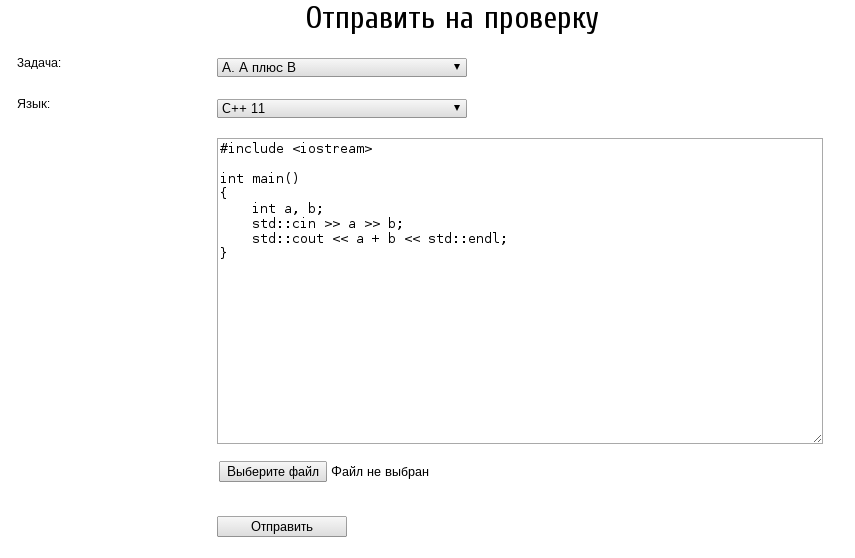
\includegraphics[width=0.8\columnwidth]{rs/sendsubmitok}
    \caption{Отправка решения}
\end{figure}

\begin{figure}[H]
    \centering
    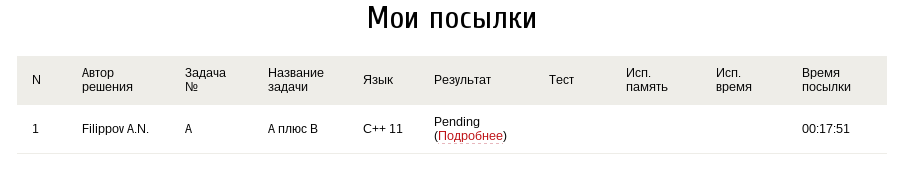
\includegraphics[width=0.8\columnwidth]{rs/mysubmitspending}
    \caption{Ожидание вынесения вердикта}
\end{figure}

\begin{figure}[H]
    \centering
    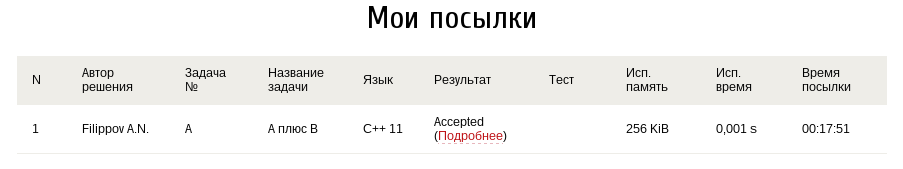
\includegraphics[width=0.8\columnwidth]{rs/mysubmitsok}
    \caption{Получение вердикта}
\end{figure}

\section{Тестирование решения с ошибками компиляции}
\begin{lstlisting}
код с ошибками компиляции
\end{lstlisting}

\begin{figure}[H]
    \centering
    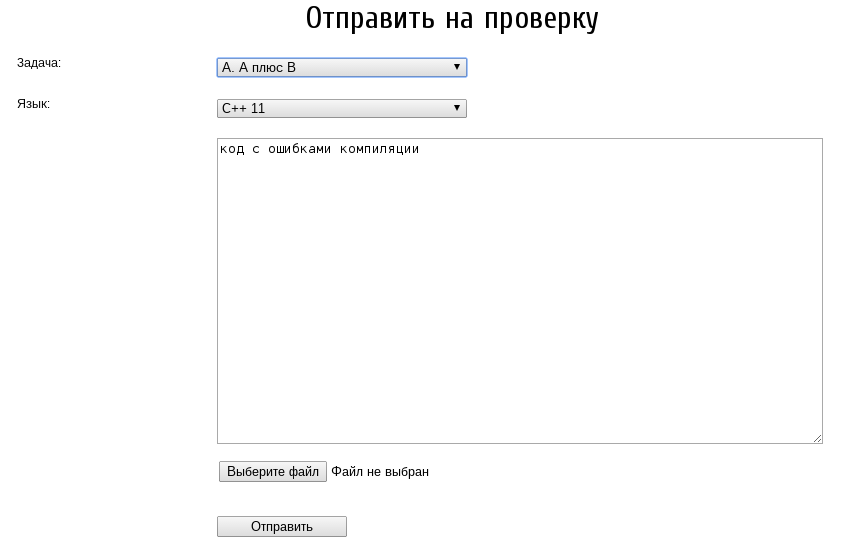
\includegraphics[width=0.8\columnwidth]{rs/sendsubmitce}
    \caption{Отправка решения}
\end{figure}

\begin{figure}[H]
    \centering
    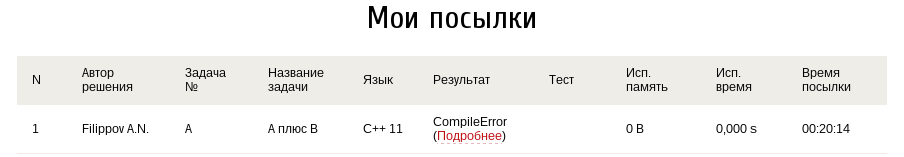
\includegraphics[width=0.8\columnwidth]{rs/mysubmitsce}
    \caption{Получение вердикта}
\end{figure}

\begin{figure}[H]
    \centering
    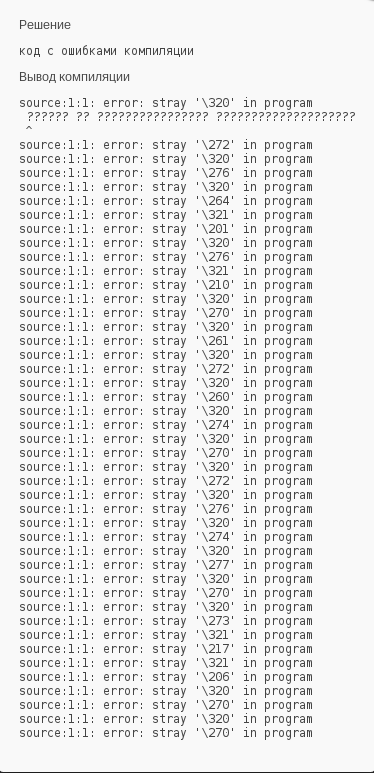
\includegraphics[width=0.5\columnwidth]{rs/mysubmitsceverbose}
    \caption{Подробная информация об ошибке компиляции}
\end{figure}

\section{Тестирование неверного решения}

\begin{lstlisting}
#include <iostream>

int main()
{
    int a, b;
    std::cin >> a >> b;
    a += b;
    if (a < 0)
        a = -a;
    std::cout << a << std::endl;
}
\end{lstlisting}

\begin{figure}[H]
    \centering
    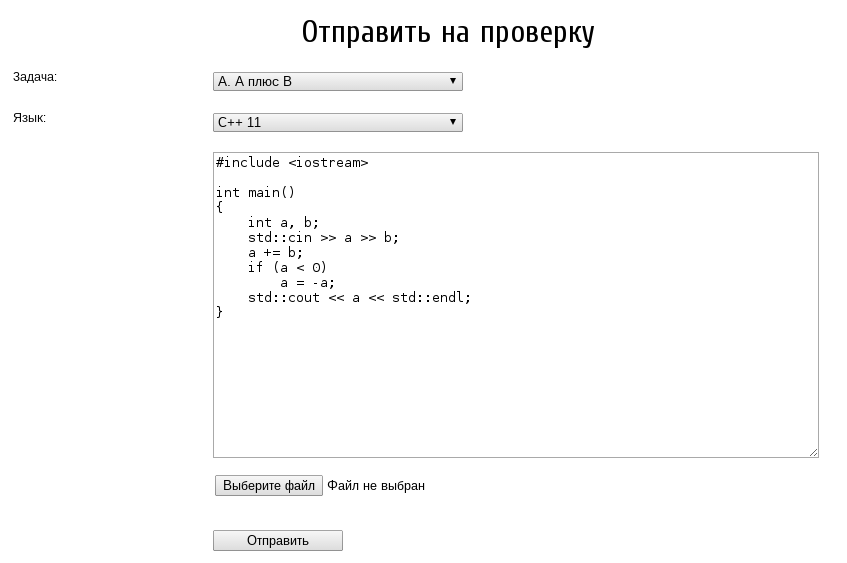
\includegraphics[width=0.8\columnwidth]{rs/sendsubmitwa}
    \caption{Отправка решения}
\end{figure}

\begin{figure}[H]
    \centering
    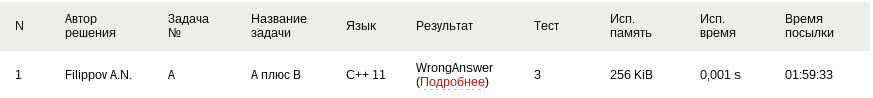
\includegraphics[width=0.8\columnwidth]{rs/mysubmitswa}
    \caption{Получение вердикта}
\end{figure}
